\documentclass[10pt]{beamer}

\usepackage{xeCJK}

\usepackage[T1]{fontenc}

\usepackage[utf8]{inputenc}

\usetheme{metropolis}
\usepackage{appendixnumberbeamer}

\usepackage{booktabs}
\usepackage[scale=2]{ccicons}

\usepackage{pgfplots}

\usepackage{xspace}

\usepackage{listings}

\lstset{
	basicstyle=\ttfamily,
	escapeinside=||
}

\usepackage{graphicx}

\newcommand{\emptyline}{\vspace{\baselineskip}}

\usepackage{ulem}


\title{程序设计教程}
\subtitle{结构体和malloc实现}
\date{2019-11-15}
\author{唐瑞泽}
\institute{tangruize@smail.nju.edu.cn}

\begin{document}

    \maketitle

    \begin{frame}{目录}
        \setbeamertemplate{section in toc}[sections numbered]
        \tableofcontents[hideallsubsections]
    \end{frame}

    \section{结构体}\label{sec:结构体}

\begin{frame}[fragile]{结构体是什么?}
    \begin{itemize}[<+- | alert@+>]
        \item 假如要存很多人的信息, 每个人信息包括姓名, 学号等, 如何存储?
        \item 我们学过数组!
        \item 那就定义很多数组: 姓名数组, 学号数组, 年龄数组\ldots
        \item 但这样太麻烦了, 如果信息很多, 代码也会变得十分难懂
        \item 要是能有一种类型, 能存一个人的所有信息就好了
        \item 结构体!
    \end{itemize}
\end{frame}

\begin{frame}[fragile]{如何定义结构体}
    \begin{itemize}[<+- | alert@+>]
        \item 结构体正如其名, 它把一组元素装进一个类型里, 元素被称为成员
        \item 语法:
        \begin{verbatim}
struct type_name {
    member_type1 member_name1;
    member_type2 member_name2;
    member_type3 member_name3;
    .
    .
} object_names;
        \end{verbatim}
        \item type\_name 是结构体的类型名, 但使用这个类型需要加上 struct
        \item object\_names 可以是用逗号隔开的多个变量名
    \end{itemize}
\end{frame}

\begin{frame}[fragile]{结构体定义示例}
    \begin{itemize}[<+- | alert@+>]
        \item 省略 object\_names, 可以用 \texttt{struct type\_name} 定义变量:
        \scriptsize\begin{verbatim}
    struct person_t {
        char name[20];
        int age;
    };
    struct person_t alice, bob;
        \end{verbatim}
        \item 可以使用 typedef 简化掉 struct:
        \scriptsize\begin{verbatim}
    typedef struct person_t person_t;
    person_t alice, bob;
        \end{verbatim}
        \item 省略 type\_name, 将不能再用该结构体定义别的变量(没有类型名):
        \scriptsize\begin{verbatim}
    struct {
        char name[20];
        int age;
    } alice, bob;
        \end{verbatim}
    \end{itemize}
\end{frame}

\begin{frame}[fragile]{访问结构体成员}
    \begin{itemize}[<+- | alert@+>]
        \item 通过点\texttt{.}访问, 即 \texttt{object\_name.member}, 举例:
        \begin{verbatim}
    alice.age = 20;
    bob.age = 22;
        \end{verbatim}
        \item 结构体指针通过\texttt{->}访问, 即 \texttt{object\_ptr->member}, 举例:
        \begin{verbatim}
    struct person_t *p = &alice;
    p->age = 20;
        \end{verbatim}
        \item \texttt{object\_ptr->member} 等价于 \texttt{(*object\_ptr).member}
    \end{itemize}
\end{frame}

\begin{frame}[fragile]{链表}
    \begin{itemize}[<+- | alert@+>]
        \item 结构体中可包含其类型的指针(但不能包含其自身), 从而形成链表:
        \begin{verbatim}
struct forward_list {
    int data;
    forward_list *next;
};
        \end{verbatim}
        \item \href{http://pythontutor.com/c.html#code=\%23include\%20\%3Cstdio.h\%3E\%0A\%23include\%20\%3Cstdlib.h\%3E\%0A\%0Astruct\%20forward_list\%20\%7B\%0A\%20\%20int\%20data\%3B\%0A\%20\%20struct\%20forward_list\%20*next\%3B\%0A\%7D\%20_head,\%20*head\%20\%3D\%20\%26_head,\%20*tail\%20\%3D\%20\%26_head\%3B\%0A\%0Atypedef\%20struct\%20forward_list\%20forward_list\%3B\%0A\%0Aint\%20main\%28\%29\%20\%7B\%0A\%20\%20for\%20\%28int\%20i\%20\%3D\%200\%3B\%20i\%20\%3C\%203\%3B\%20\%2B\%2Bi\%29\%20\%7B\%0A\%20\%20\%20\%20tail-\%3Enext\%20\%3D\%20\%28forward_list\%20*\%29malloc\%28sizeof\%28forward_list\%29\%29\%3B\%0A\%20\%20\%20\%20tail\%20\%3D\%20tail-\%3Enext\%3B\%0A\%20\%20\%20\%20tail-\%3Edata\%20\%3D\%20i\%3B\%0A\%20\%20\%20\%20tail-\%3Enext\%20\%3D\%20NULL\%3B\%0A\%20\%20\%7D\%0A\%20\%20for\%20\%28forward_list\%20*p\%20\%3D\%20head-\%3Enext,\%20*q\%20\%3D\%20p\%3B\%20p\%20!\%3D\%20NULL\%3B\%20q\%20\%3D\%20p\%29\%20\%7B\%0A\%20\%20\%20\%20printf\%28\%22\%25d\%5Cn\%22,\%20p-\%3Edata\%29\%3B\%0A\%20\%20\%20\%20p\%20\%3D\%20p-\%3Enext\%3B\%0A\%20\%20\%20\%20free\%28q\%29\%3B\%0A\%20\%20\%20\%20head-\%3Enext\%20\%3D\%20p\%3B\%0A\%20\%20\%20\%20if\%20\%28tail\%20\%3D\%3D\%20q\%29\%0A\%20\%20\%20\%20\%20\%20tail\%20\%3D\%20head\%3B\%0A\%20\%20\%7D\%0A\%7D&mode=edit&origin=opt-frontend.js&py=c&rawInputLstJSON=\%5B\%5D}{可视化样例}
    \end{itemize}
\end{frame}

\begin{frame}[fragile]{双向链表}
    \begin{itemize}[<+- | alert@+>]
        \item forward\_list 只能向后遍历, 不能向前
        \item 如果在链表中间插入删除元素, 需要维护前一个结点的next信息, forward\_list 难以高效插入删除
        \item 多加一个指向前一个结点的指针不就好了!
        \item 于是我们得到了双向链表, 这是计算机中用空间换时间的典型案例
        \begin{verbatim}
struct list {
    int data;
    struct list *previous;
    struct list *next;
};
        \end{verbatim}
        \item \href{http://pythontutor.com/c.html#code=\%23include\%20\%3Cstdio.h\%3E\%0A\%23include\%20\%3Cstdlib.h\%3E\%0A\%0Astruct\%20list\%20\%7B\%0A\%20\%20int\%20data\%3B\%0A\%20\%20struct\%20list\%20*previous\%3B\%0A\%20\%20struct\%20list\%20*next\%3B\%0A\%7D\%20_head,\%20*head\%20\%3D\%20\%26_head,\%20*tail\%20\%3D\%20\%26_head\%3B\%0A\%0Atypedef\%20struct\%20list\%20list\%3B\%0A\%0Avoid\%20insert_node\%28list\%20*p,\%20int\%20data\%29\%20\%7B\%0A\%20\%20list\%20*node\%20\%3D\%20\%28list\%20*\%29malloc\%28sizeof\%28list\%29\%29\%3B\%0A\%20\%20node-\%3Edata\%20\%3D\%20data\%3B\%0A\%20\%20node-\%3Eprevious\%20\%3D\%20p\%3B\%0A\%20\%20node-\%3Enext\%20\%3D\%20p-\%3Enext\%3B\%0A\%20\%20if\%20\%28p-\%3Enext\%29\%0A\%20\%20\%20\%20p-\%3Enext-\%3Eprevious\%20\%3D\%20node\%3B\%0A\%20\%20else\%0A\%20\%20\%20\%20tail\%20\%3D\%20node\%3B\%0A\%20\%20p-\%3Enext\%20\%3D\%20node\%3B\%0A\%7D\%0A\%0Avoid\%20delete_node\%28list\%20*p\%29\%20\%7B\%0A\%20\%20p-\%3Eprevious-\%3Enext\%20\%3D\%20p-\%3Enext\%3B\%0A\%20\%20if\%20\%28p-\%3Enext\%29\%0A\%20\%20\%20\%20p-\%3Enext-\%3Eprevious\%20\%3D\%20p-\%3Eprevious\%3B\%0A\%20\%20else\%0A\%20\%20\%20\%20tail\%20\%3D\%20p-\%3Eprevious\%3B\%0A\%20\%20free\%28p\%29\%3B\%0A\%7D\%0A\%0Aint\%20main\%28\%29\%20\%7B\%0A\%20\%20for\%20\%28int\%20i\%20\%3D\%200\%3B\%20i\%20\%3C\%203\%3B\%20\%2B\%2Bi\%29\%0A\%20\%20\%20\%20insert_node\%28tail,\%20i\%29\%3B\%0A\%20\%20for\%20\%28list\%20*p\%20\%3D\%20head-\%3Enext\%3B\%20p\%20!\%3D\%20NULL\%3B\%20p\%20\%3D\%20p-\%3Enext\%29\%0A\%20\%20\%20\%20printf\%28\%22\%25d\%5Cn\%22,\%20p-\%3Edata\%29\%3B\%0A\%20\%20delete_node\%28head-\%3Enext-\%3Enext\%29\%3B\%0A\%20\%20delete_node\%28tail\%29\%3B\%0A\%20\%20delete_node\%28head-\%3Enext\%29\%3B\%0A\%7D\%0A&mode=edit&origin=opt-frontend.js&py=c&rawInputLstJSON=\%5B\%5D}{可视化样例}
    \end{itemize}
\end{frame}

    \section{malloc实现}\label{sec:malloc实现}

\begin{frame}[fragile]{一些问题?}
    \begin{itemize}[<+- | alert@+>]
        \item 能不能 free() 一部分, 比如 malloc() 得到的 ptr, \texttt{free(ptr + 1)}?
        \item 能不能 free() 不是 malloc() 得到的指针?
        \item 能不能 free() 同一个指针两次?
        \item 好像越界一点点没问题?
        \item 需要知道一些 malloc() 实现的细节!
        \item 点击下载 \href{http://problemoverflow.top/download/my\_malloc.zip}{my\_malloc.zip}
    \end{itemize}
\end{frame}

\begin{frame}[fragile]{malloc实现细节}
    链表.
\end{frame}

\begin{frame}[fragile]{malloc实现细节}
    malloc():
    \begin{itemize}[<+- | alert@+>]
        \item 从双向链表 free\_list 中找到一个合适大小的 chunk
        \item 找不到就向系统申请一块空间, 将多申请的空间放入 free\_list 中, 返回申请到的内存的某个位置的指针
        \item 找到了, 先看 chunk 能不能拆分, 能拆就取一部分出来返回(以节约内存), 不能拆就把整个 chunk 返回
    \end{itemize}
    free():
    \begin{itemize}[<+- | alert@+>]
        \item 如果参数 ptr 不为NULL, 则将 ptr 放回 free\_list 以回收利用
        \item 如果放回后有 chunk 能合并, 则合并以减少内存碎片化
    \end{itemize}
\end{frame}

\begin{frame}[fragile]{free\_list}
    \scriptsize\begin{verbatim}
struct my_malloc_chunk {
    size_t unused;
    size_t size;
    struct my_malloc_chunk *previous;
    struct my_malloc_chunk *next;
} *free_list;
    \end{verbatim}
    free\_list 为类型为 my\_malloc\_chunk* 的链表头指针, 为 NULL 表示没有分配的内存
    \begin{figure}[ht!]
        \centering
        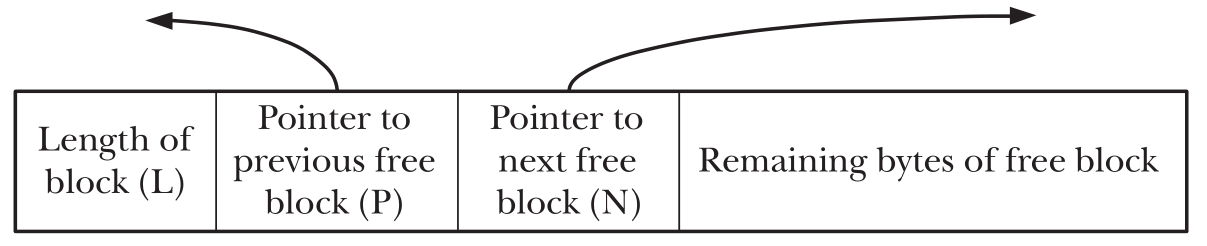
\includegraphics[width=60mm]{figs/my_malloc_chunk.png}
        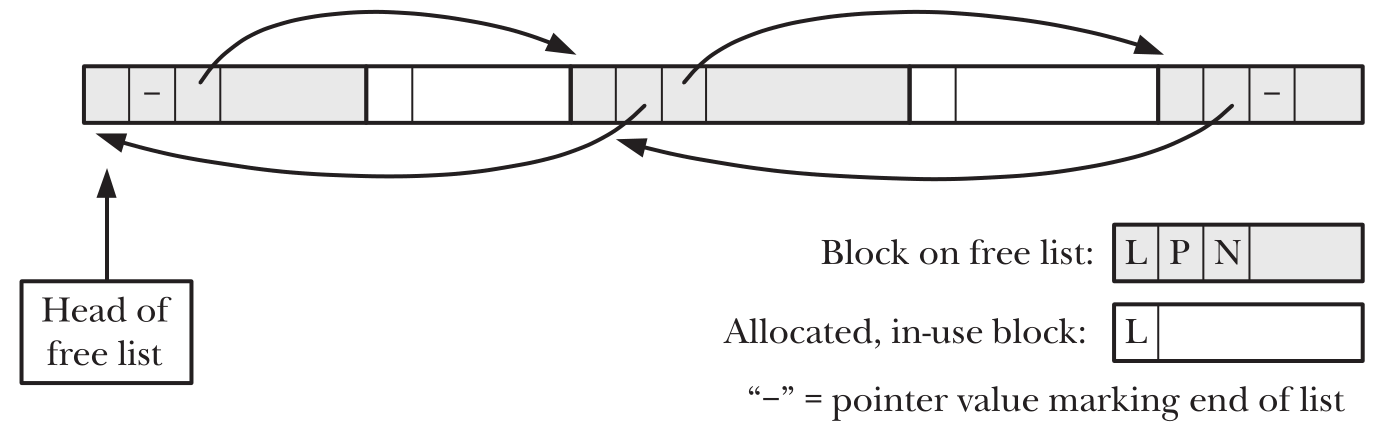
\includegraphics[width=80mm]{figs/free_list.png}
        \caption{free\_list}
    \end{figure}
\end{frame}

\begin{frame}[fragile]{向系统申请空间}
    \begin{itemize}[<+- | alert@+>]
        \item 程序能申请增大或减小堆空间大小
        \item 堆位于未初始化数据区域, 当前的限制称为 program break (可以理解为一个指针)
        \item 增加或减小堆大小, 系统只要相应地提升或降低 program break 指向位置即可
        \item brk() 和 sbrk() 系统调用用来做这件事
    \end{itemize}
\end{frame}

\begin{frame}[fragile]{向系统申请空间}
    \small\begin{verbatim}
#include <unistd.h>

int brk(void * end_data_segment);
    // Returns 0 on success, or –1 on error

void *sbrk(intptr_t increment);
    // Returns previous program break on success,
    // or (void *) –1 on error
    \end{verbatim}
\end{frame}

\begin{frame}[fragile]{malloc实验教程}
    \begin{itemize}[<+- | alert@+>]
        \item 下载 \href{http://problemoverflow.top/download/my\_malloc.zip}{my\_malloc.zip}, 解压后在 CLion 打开.
        \item 由于使用了 Windows 不原生支持的 sbrk() 等函数, 请在 Linux 环境或 Cygwin 环境下进行实验 (MinGW 不能用)
        \item 编译运行test, 程序使用的标准库 malloc()
        \item 在 test.c 中找到并取消注释 \texttt{//\#define USE\_MY\_MALLOC}
        \item 编译运行test, 程序给出提示并异常退出
        \item TODO: 你需要在 my\_malloc.c 文件实现 allocate\_more\_chunk() 相关代码
    \end{itemize}
\end{frame}

\begin{frame}[fragile]{malloc实验教程}
    \begin{itemize}[<+- | alert@+>]
        \item 编译运行test, 程序正常执行, 对比使用标准库 malloc() 的输出
        \item 我们的程序使用了很大的内存
        \item 原因是从 free\_list 删除一个结点时直接把 free\_list 赋为 NULL, 已申请的空间全部不能回收利用
        \item TODO: 实现 delete\_from\_free() 相关代码
    \end{itemize}
\end{frame}

\begin{frame}[fragile]{malloc实验教程}
    \begin{itemize}[<+- | alert@+>]
        \item 编译运行test, 程序用的内存减少, 但仍然很多
        \item 程序没有对大块的内存进行切分
        \item TODO: 实现 get\_pointer() 相关代码
    \end{itemize}
\end{frame}

\begin{frame}[fragile]{malloc实验教程}
    \begin{itemize}[<+- | alert@+>]
        \item 编译运行test, 根据你实现的不同, 程序运行起来可能超级慢! 而且内存使用不降反增!
        \item 对内存切分造成了许多小的内存碎片, 这些碎片难以分配出去且使得链表变长
        \item 搜索 chunk 时如果有刚好相同或差不多大小的 chunk, 切分时可减少内存碎片
        \item TODO: 实现 find\_fit\_chunk() 相关代码, 使用best-fit搜索策略
    \end{itemize}
\end{frame}

\begin{frame}[fragile]{malloc实验教程}
    \begin{itemize}[<+- | alert@+>]
        \item 编译运行test, 程序变快了, 内存使用也减少了, 但运行仍然太慢
        \item 内存碎片仍没有得到有效解决, 代码只切分 chunk 而很少合并
        \item TODO: 实现 add\_to\_free() 相关代码, 改进加入链表和合并策略
    \end{itemize}
\end{frame}

\begin{frame}[fragile]{malloc实验教程}
    \begin{itemize}[<+- | alert@+>]
        \item 编译运行test, 程序又变快了很多, 内存使用量也变得稳定, 虽然运行速度仍远远比不上标准库
        \item 还有什么可以改进的地方?
        \item 机器对地址对齐的数据处理较快
        \item TODO: 实现 request\_size() 相关代码, 满足对齐要求
    \end{itemize}
\end{frame}

\begin{frame}[fragile]{malloc实验教程}
    \begin{itemize}[<+- | alert@+>]
        \item 编译运行test, 速度只得到了小幅改进
        \item 还有什么可以改进的地方?
        \item 编译gprof, 查看函数调用执行时间和占比, 进一步优化你的程序
        \item 更多可实现的地方请参看源代码 TODO advanced
    \end{itemize}
\end{frame}

\begin{frame}[fragile]{一些问题还有吗?}
    \begin{itemize}[<+- | alert@+>]
        \item 能不能 free() 一部分, 比如 malloc() 得到的 ptr, \texttt{free(ptr + 1)}?
        \item 能不能 free() 不是 malloc() 得到的指针?
        \item 能不能 free() 同一个指针两次?
        \item 好像越界一点点没问题?
    \end{itemize}
\end{frame}

    \begin{frame}[standout]
        Questions?
    \end{frame}

\end{document}
